%common derivatives and integrals, and substitutions
\date{}
\documentclass[fleqn, a4paper, 10pt]{article}
\usepackage[top=1.5cm, left=1.5cm, right=1.5cm, inner = 2cm]{geometry}
\usepackage{amsmath, amssymb, amsthm} %standard AMS packages
\usepackage{commath, esdiff} %typesetting differentials
\usepackage{gensymb}
\usepackage{hyperref} %hyperlinking
\usepackage{tikz, pgfplots} %drawing figures
\usepackage{datetime} % formatting dates
\usepackage{ulem} %change \emph to underline
\usepackage{enumerate, enumitem} %numbered list and formatting 
\usepackage{multicol}
\usepackage{thmtools}

\setcounter{secnumdepth}{4} %numbering \paragraph

\newcommand\numberthis{\addtocounter{equation}{1}\tag{\theequation}} %reset 

\theoremstyle{definition}
\newtheorem{example}{Example}
\newtheorem{definition}{Definition}

\theoremstyle{theorem}
\newtheorem{theorem}{Theorem}

\theoremstyle{remark}
\newtheorem{remark}{Remark}
\newtheorem{case}{Case}

\newenvironment{solution}
	{\begin{proof}[Solution]\let\qed\relax}
	{\end{proof}}

%%section headings on left
%\makeatletter
%\def\specialsection{\@startsection{section}{1}%
%	\z@{\linespacing\@plus\linespacing}{.5\linespacing}%
%	%  {\normalfont\centering}}% DELETED
%	{\normalfont}}% NEW
%\def\section{\@startsection{section}{1}%
%	\z@{.7\linespacing\@plus\linespacing}{.5\linespacing}%
%	%  {\normalfont\scshape\centering}}% DELETED
%	{\normalfont\scshape}}% NEW
%\makeatother
%
%%forces newline after subsection
%\makeatletter
%\def\subsection{\@startsection{subsection}{3}%
%	\z@{.5\linespacing\@plus.7\linespacing}{.1\linespacing}%
%	{\normalfont\itshape}}
%\makeatother

%opening
\title{Differential and Integral Methods: Compendium}
\author{Aakash Jog}

\begin{document}
	
\maketitle
\setlength{\mathindent}{0pt}

\tableofcontents

\vspace{1cm}
\hrule
\vspace{1cm}

\begin{multicols}{2}

\section{Functions}

\begin{definition}[Even function]
	\begin{equation*}
		f(-x) = f(x)
	\end{equation*}
\end{definition}

\begin{definition}[Odd function]
	\begin{equation*}
	f(-x) = -f(x)
	\end{equation*}
\end{definition}

\subsection{Hyperbolic Functions}

\begin{definition}[Hyperbolic functions]
	\begin{align*}
		\sinh x &\dot{=} \dfrac{e^x - e^{-x}}{2}
		& I(\sinh x) &= \mathbb{R}\\
		\cosh x &\dot{=} \dfrac{e^x + e^{-x}}{2}
		& I(\cosh x) &= [1, \infty)\\
		\tanh x &\dot{=} \dfrac{\sinh x}{\cosh x} = \dfrac{e^x - e^{-x}}{e^x + e^{-x}}
		& I(\tanh x) &= (-1, 1)
	\end{align*}
\end{definition}

\subsubsection{Identities of Hyperbolic Functions}

\begin{align*}
	\sinh (2x) &= 2 \sinh x \cosh x \\
	\cosh ^2 x + \sinh ^2 x &= \cosh (2x) \\
	\cosh ^2 x - \sinh ^2 x &= 1 \\
	\dfrac{\cosh (2x) - 1}{2} &= \sinh ^2 x \\
	\dfrac{\cosh (2x) + 1}{2} &= \cosh ^2 x 
\end{align*}

\subsection{Trigonometric Identities}

\begin{align*}
	\sin^2 x + \cos^2 x &= 1\\
	\tan^2 x + 1 &= \sec^2 x\\
	\cot^2 x + 1 &= \csc^2 x
\end{align*}

\begin{align*}
	\sin(x \pm y) &= \sin x \cos y \pm \cos x \sin y\\
	\cos(x \pm y) &= \cos x \cos y \mp \sin x \sin y\\
	\tan(x \pm y) &= \dfrac{\tan x \pm \tan y}{1 \mp \tan x \tan y}
\end{align*}

\begin{align*}
	\sin x \sin y &= \dfrac{1}{2} \left( \cos(x - y) - \cos(x + y) \right)\\
	\cos x \cos y &= \dfrac{1}{2} \left( \cos(x - y) + \cos(x + y) \right)\\
	\sin x \cos y &= \dfrac{1}{2} \left( \sin(x + y) + \sin(x - y) \right)\\
	\cos x \sin y &= \dfrac{1}{2} \left( \sin(x + y) - \sin(x - y) \right)
\end{align*}

\begin{align*}
	\sin x + \sin y &= 2 \sin \left( \dfrac{x + y}{2} \right) \cos \left( \dfrac{x - y}{2} \right)\\
	\sin x - \sin y &= 2 \cos \left( \dfrac{x + y}{2} \right) \sin \left( \dfrac{x - y}{2} \right)\\
	\cos x + \cos y &= 2 \cos \left( \dfrac{x + y}{2} \right) \cos \left( \dfrac{x - y}{2} \right)\\
	\cos x - \cos y &= -2 \sin \left( \dfrac{x + y}{2} \right) \sin \left( \dfrac{x - y}{2} \right)
\end{align*}

\begin{align*}
	\sin \dfrac{x}{2} &= \pm \sqrt{\dfrac{1 - \cos x}{2}}\\
	\cos \dfrac{x}{2} &= \pm \sqrt{\dfrac{1 + \cos x}{2}}\\
	\tan \dfrac{x}{2} &= \pm \sqrt{\dfrac{1 - \cos x}{1 + \cos x}}
\end{align*}

\section{Limits}

\begin{definition}[Cauchy's definition of a limit of a function]
	\begin{equation*}
	\forall \epsilon > 0 \exists \delta > 0 : 0 < |x - a| < \delta \Rightarrow |f(x) - L| < \epsilon
	\end{equation*}
\end{definition}

\begin{definition}[Removable discontinuity point]
	\begin{equation*}
		\exists \lim\limits_{x \rightarrow a} f(x)$, but either $\lim\limits_{x \rightarrow a} f(x) \neq f(a)$ or $\nexists f(a)
	\end{equation*}
\end{definition}

\begin{definition}[Discontinuity of first kind]
	\begin{equation*}
		\exists \lim\limits_{x \rightarrow a^-} f(x), \exists \lim\limits_{x \rightarrow a^+} f(x)$, but $\lim\limits_{x \rightarrow a^-} f(x) \neq \lim\limits_{x \rightarrow a^+} f(x)
	\end{equation*}
\end{definition}

\begin{definition}[Discontinuity of second kind]
	At least one of the two one-sided limits of $f$ does not exist. (Limits are defined as finite numbers only.)
\end{definition}

\begin{theorem}[Sandwich Theorem] \label{Sandwich Theorem}
	Let $f(x), g(x), h(x)$ be defined on an open interval about $a$, except possibly at $a$ itself. Assume that $\forall x \neq a$ from the interval, it is satisfied that $f(x) \leq g(x) \leq h(x)$ and $\lim\limits_{x \rightarrow a} f(x) = \lim\limits_{x \rightarrow a} h(x) = L$. Then, 
	\begin{equation*}
		\lim\limits_{x \rightarrow a} g(x) = L
	\end{equation*}
\end{theorem}

\begin{theorem}
	If $\lim\limits_{x \rightarrow a} f(x) = 0$ and $g(x)$ is bounded in an open interval about $a$, except possibly at $a$ itself, then, 
	\begin{equation*}
		\lim\limits_{x \rightarrow a}(f(x)g(x)) = 0
	\end{equation*}
\end{theorem}

\subsection{Useful Limits}

If $\lim\limits_{x \rightarrow x_0} g(x) = 0$, 
\begin{equation*}
	\lim\limits_{x \rightarrow x_0} (1 + g(x))^{\frac{1}{g(x)}} = e
\end{equation*}

\begin{align*}
	\lim\limits_{x \rightarrow +\infty} \left(1 + \dfrac{1}{x}\right) ^x &= e\\
	\lim\limits_{x \rightarrow -\infty} \left(1 + \dfrac{1}{x}\right) ^x &= e\\
	\lim\limits_{\theta \rightarrow 0} \dfrac{\sin \theta}{\theta} &= 1
\end{align*}

\section{Derivatives}

\begin{definition}[Derivative of a function]
	\begin{equation*}
		\dod{y}{x} = \lim\limits_{\Delta x \rightarrow 0} \dfrac{f(x_0 + \Delta x) - f(x_0)}{\Delta x} = L
	\end{equation*}
\end{definition}

\begin{theorem}[Derivative of inverse functions]
	\begin{equation*}
	(f^{-1})'(x) = \dfrac{1}{f'(x)}
	\end{equation*}
\end{theorem}

\begin{theorem}[Chain rule]
	\begin{equation*}
	\dod{f(g(x))}{x} = \dod{f(g(x))}{g(x)} \cdot \dod{g(x)}{x}
	\end{equation*}
\end{theorem}

\begin{theorem}[Rolle's Theorem]
	Let $f(x)$ be defined on $[a, b]$, s.t. 
	\begin{enumerate}
		\item $f$ is continuous on $[a, b]$ \label{Rolle condition 1}
		\item $f$ is differentiable on $(a, b)$ \label{Rolle condition 2}
		\item $f(a) = f(b)$ \label{Rolle condition 3}
	\end{enumerate}
	Then, $\exists c \in (a, b)$, s.t. $f'(c) = 0$.
\end{theorem}

\begin{theorem}[Lagrange Theorem]
	Let $f(x)$ be defined on $[a, b]$, s.t. 
	\begin{enumerate}
		\item $f$ is continuous on $[a, b]$
		\item $f$ is differentiable on $(a, b)$
	\end{enumerate}
	Then, 
	\begin{equation*}
		\exists c \in (a, b)$, s.t. $f'(c) = \dfrac{f(b) - f(a)}{b - a}
	\end{equation*}
\end{theorem}

\section{Taylor's Formula}

\begin{theorem}[Taylor's Formula]
	\begin{align*}
		f(x) &= \sum_{i = 0}^{n} \dfrac{f^{(i)}(a)}{i!} (x - a)^i + \dfrac{f^{(n)}(c)}{(n+1)!} (x-a)^{n+1}
	\end{align*}
\end{theorem}

\subsection{Common Derivatives}

\begin{gather*}
\dod{}{x} x = 1\\
\dod{}{x} \sin x = \cos x\\
\dod{}{x} \cos x = - \sin x\\
\dod{}{x} \tan x = \sec^2 c\\
\dod{}{x} \sec x = \sec x \tan x\\
\dod{}{x} \csc x = - \csc x \cot x\\
\dod{}{x} \cot x = - \csc^2 c\\
\dod{}{x} \sin^{-1} x = \dfrac{1}{\sqrt{1 - x^2}}\\
\dod{}{x} \cos^{-1} x = -\dfrac{1}{\sqrt{1 - x^2}}\\
\dod{}{x} \tan^{-1} x = \dfrac{1}{1 + x^2}\\
\dod{}{x} a^x = a^x \ln a\\
\dod{}{x} \ln x = \dfrac{1}{x}\\
\dod{}{x} \log_{a} x = \dfrac{1}{x \ln a}
\end{gather*}

\section{Full Investigation of Functions}

\begin{enumerate}
	\item Domain of definition of $f$
	\item Points of intersection of $y = f(x)$ with $x$-axis and $y$-axis
	\item Symmetry and periodicity
	\item Extrema points
	\item Monotonicity
	\item Convexity
	\item Inflection points
	\item Asymptotes (vertical and oblique)
	\item Graph
\end{enumerate}

\begin{definition}[Vertical asymptote]
	Let $f(x)$ be defined on $(a - \delta)$ or $(a, a + \delta)$ or $(a - \delta, a + \delta) - \{a\}$ for $\delta > 0$. If atleast one of $\lim\limits_{x \to a^-} f(x)$ and $\lim\limits_{x \to a^+} f(x)$ is equal to $\pm \infty$, then the straight line $x = a$ is said to be a vertical asymptote of $f(x)$.
\end{definition}

\begin{definition}[Oblique asymptote]
	The straight line $y = ax + b$ is called an oblique asymptote of a function $y = f(x)$ at $+ \infty$ (or $- \infty$), if 
	\begin{align*}
		\lim\limits_{x \to + \infty} (f(x) - (ax+b)) &= 0 \\
		\Big( \text{ or } \lim\limits_{x \to -\infty} (f(x) - (ax+b)) &= 0 \Big)
	\end{align*}
\end{definition}

\begin{example}
	Investigate
	\begin{equation*}
	y = f(x) =\dfrac{(x-1)^3}{(x+1)^2}
	\end{equation*}
\end{example}

\begin{solution}
	\begin{align*}
		D(f) &= \mathbb{R} - \{-1\}
	\end{align*}
	\begin{align*}
		y &= 0 &\implies x &= 1\\
		x &= 0 &\implies y &= -1
	\end{align*}
	The function is not periodic.
	\begin{align*}
		f(-x) &\neq f(x) \\
		&\neq -f(x) 
	\end{align*}
	Therefore, the function is not symmetric.
	\begin{align*}
		f'(x) &= \dfrac{(x-1)^2 (x+5)}{(x+1)^3}
	\end{align*}
	Therefore, $x = -5$ is a local maximum point.\\
	The function is monotonically increasing in $(-\infty, -5) \cup (-1, +\infty)$ and is monotonically decreasing in $(-5, -1)$.
	\begin{align*}
		f''(x) &= \dfrac{24(x-1)}{(x+1)^4}
	\end{align*}
	Therefore, the function is convex upwards in $(-\infty, -1) \cup (-1, 1)$ and convex downwards in $(1, \infty)$.
	\begin{align*}
		\lim\limits_{x \to -1^-} \dfrac{(x-1)^3}{(x+1)^2} &= \dfrac{-8}{+0}\\
		&= -\infty\\
		\lim\limits_{x \to -1^+} \dfrac{(x-1)^3}{(x+1)^2} &= \dfrac{-8}{+0}\\
		&= -\infty
	\end{align*}
	Therefore, $x = -1$ is a vertical asymptote of $f(x)$.
	\begin{align*}
		a_1 &= \lim\limits_{x \to +\infty} \dfrac{f(x)}{x} &= 1\\
		b_1 &= \lim\limits_{x \to +\infty} \left(f(x) - a_1 x\right) &= -5\\
		a_2 &= \lim\limits_{x \to -\infty} \dfrac{f(x)}{x} &= 1\\
		b_2 &= \lim\limits_{x \to -\infty} \left(f(x) - a_1 x\right) &= -5
	\end{align*}
	Therefore, $y = x - 5$ is an oblique asymptote of the function, at $+\infty$ and $-\infty$.
\end{solution}

\section{Integration}

\begin{definition}[Basic rational functions]
	A simple rational function of one of the following forms is called a basic rational function.
	\begin{align*}
		\dfrac{A}{x - \alpha} &\quad; A, \alpha \in \mathbb{R}\\
		\dfrac{A}{(x - \alpha)^n} &\quad; A, \alpha \in \mathbb{R}, n \in \mathbb{N} - \{1\}\\
		\dfrac{Ax +  B}{x^2 + px + q} &\quad; A, B, p, q \in \mathbb{R}, p^2 - 4q < 0\\
		\dfrac{Ax + B}{(x^2 + px + q)^n} &\quad; A, B, p, q \in \mathbb{R}, p^2 - 4q < 0, n \in \mathbb{N} - \{1\}
	\end{align*}
\end{definition}

\begin{example}
	Solve $\displaystyle \int \dfrac{-x + 2}{x(x - 1)^2} \dif x$.
\end{example}

\begin{solution}
	\begin{align*}
		\int \dfrac{-x + 2}{x(x - 1)^2} \dif x &= \int \left(\dfrac{A_1}{x} + \dfrac{B_1}{x - 1} + \dfrac{B_2}{(x - 1)^2}\right) \dif x
	\end{align*}
	\begin{align*}
		\dfrac{-x + 2}{x(x - 1)^2} &= \dfrac{A_1 (x - 1)^2 + B_1 (x)(x - 1) + B_2 x}{x(x - 1)^2}\\
		&= \dfrac{x^2(A_1 + B_1) + x(-2A_1 - B_1 + B_2) + A_1}{x(x - 1)^2}
	\end{align*}
	Therefore,
	\begin{align*}
		A_1 + B_1 &= 0\\
		-2A_1 - B_1 + B_2 &= -1\\
		A_1 &= 2
	\end{align*}
	Therefore, 
	\begin{align*}
		A_1 &= 2\\
		B_1 &= -2\\
		B_2 &= 1
	\end{align*}
	Therefore,
	\begin{align*}
		\int \dfrac{-x + 2}{x(x - 1)^2} \dif x &= \int \left(\dfrac{2}{x} + \dfrac{-2}{x - 1} + \dfrac{1}{(x - 1)^2}\right) \dif x\\
		&= 2 \ln |x| - 2 \ln |x - 1| - \dfrac{1}{x - 1} + c\\
		&= 2 \ln \left|\dfrac{x}{x - 1}\right| - \dfrac{1}{x - 1} + x
	\end{align*}
\end{solution}

\begin{example}
	Solve $\displaystyle \int \dfrac{2x^2 - x + 4}{x^3 + 4x} \dif x$.
\end{example}

\begin{solution}
	\begin{align*}
		\int \dfrac{2x^2 - x + 4}{x^3 + 4x} \dif x &= \int \dfrac{2x^2 - x + 4}{x(x^2 + 4)} \dif x\\
		&= \int \left(\dfrac{A}{x} + \dfrac{Bx + C}{x^2 + 4}\right) \dif x\\
		\dfrac{2x^2 - x + 4}{x^3 + 4x} &= \dfrac{A(x^2 + 4) + (Bx + c)x}{x(x^2 + 4)}\\
		&= \dfrac{x^2(A + B) + x(C) + 4A}{x(x^2 + 4)}
	\end{align*}
	Therefore,
	\begin{align*}
		A + B &= 2\\
		C &= -1\\
		4A &= 4
	\end{align*}
	Therefore, 
	\begin{align*}
		A &= 1\\
		B &= 1\\
		C &= -1
	\end{align*}
	Therefore,
	\begin{align*}
		\int \dfrac{2x^2 - x + 4}{x(x^2 + 4)} \dif x &= \int \left(\dfrac{1}{x} + \dfrac{x - 1}{x^2 + 4}\right) \dif x\\
		&= \ln |x| \\
		&\quad+ \int \dfrac{x}{x^2 + 4} \dif x - \int \dfrac{1}{x^2 + 4} \dif x + d\\
		&= \ln |x|\\
		&\quad+ \dfrac{1}{2} \ln (x^2 + 4) - \dfrac{1}{2}\arctan\left(\dfrac{x}{2}\right) + d
	\end{align*}
\end{solution}

\begin{theorem}[Integration by Parts]
	\begin{align*}
		\int u v \dif x &= u \int v \dif x - \int u' \left(\int v \dif x\right) \dif x
	\end{align*}
\end{theorem}

\begin{theorem}[Fundamental Theorem of Calculus, Part 1]\label{Fundamental Theorem of Calculus, Part 1}
	Let $f(x)$ be continuous on $(a, b)$ and let $c \in (a, b)$. Then, the function $F(x) = \int\limits_{c}^{x} f(t) \dif t$ is an anti-derivative function of $f(x)$ on $(a, b)$, i.e.
	\begin{equation*}
	F'(x) = f(x) \quad ; \quad \forall x \in (a, b)
	\end{equation*}
\end{theorem}

\begin{theorem}[Fundamental Theorem of Calculus, Part 2]
	Let $f(x)$ be continuous on $[a, b]$ and let $G(x)$ be an arbitrary anti-derivative function of $f(x)$. Then,
	\begin{equation*}
	\int\limits_{a}^{b} f(x) \dif x = G(b) - G(a)
	\end{equation*}
\end{theorem}

\subsection{Common Integrals}

\begin{gather*}
	\int k \dif x = kx + c\\
	\int x^n \dif x = 
		\begin{cases}
			\dfrac{1}{n + 1} x^{n + 1} + c &; \quad n \neq -1\\
			\ln |x| + c &;\quad n = -1\
		\end{cases}\\
	\int \dfrac{1}{a x + b} \dif x = \dfrac{1}{a} \ln |a x + b| + c\\
	\int \ln x \dif x = x \ln x - x + c\\
	\int e^x \dif x = e^x + c\\
	\int \cos x \dif x = \sin x + c\\
	\int \sin x \dif x = - \cos x + c\\
	\int \sec^2 x \dif x = \tan x + c\\
	\int \csc^2 x \dif x = -\cot x + c\\
	\int \sec x \tan x \dif x = \sec x + c\\
	\int \csc x \cot x \dif x = -\csc x + c\\
	\int \tan x \dif x = \ln |\sec x| + c\\
	\int \sec x \dif x = \ln |\sec x + \tan x| + c\\
	\int \dfrac{1}{a^2 + x^2} \dif x = \dfrac{1}{a} \tan^{-1} \dfrac{x}{a} + c\\
	\int \dfrac{1}{\sqrt{a^2 - x^2}} \dif x = \sin^{-1} \dfrac{x}{a} + c
\end{gather*}

\subsection{Length of a Curve}

\begin{align*}
	l &= \int\limits_{a}^{b} \sqrt{1 + (f'(x))^2} \dif x
\end{align*}

\subsection{Volume of Solids of Rotation}

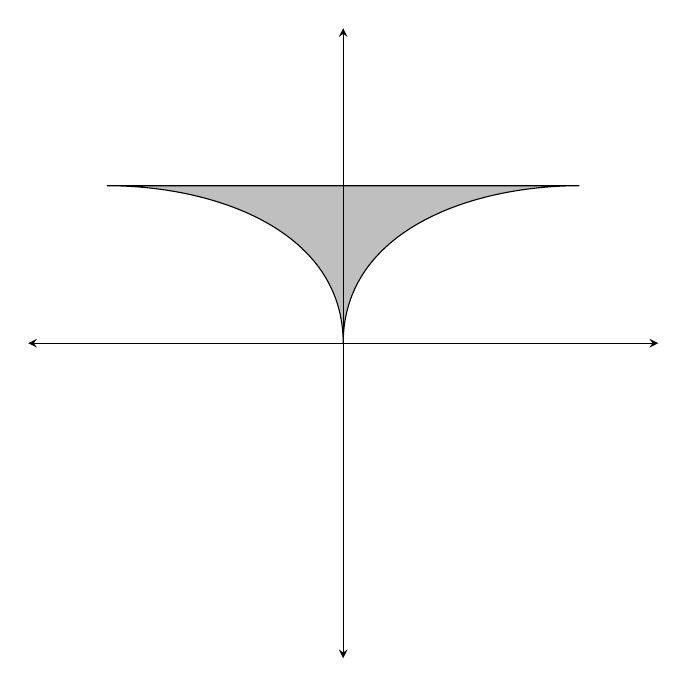
\begin{tikzpicture}
	\draw [fill = lightgray] (-3,2) [out = 0, in = 90] to (0,0) [out = 90, in = 180] to (3,2) -- cycle;
	
	\begin{scope}[stealth-stealth]
		\draw (-4,0) -- (4,0);
		\draw (0,-4) -- (0,4);
	\end{scope}
\end{tikzpicture}

\begin{equation*}
	V = \pi \int\limits_{a}^{b} \left( f(y) \right)^2 \dif y
\end{equation*}

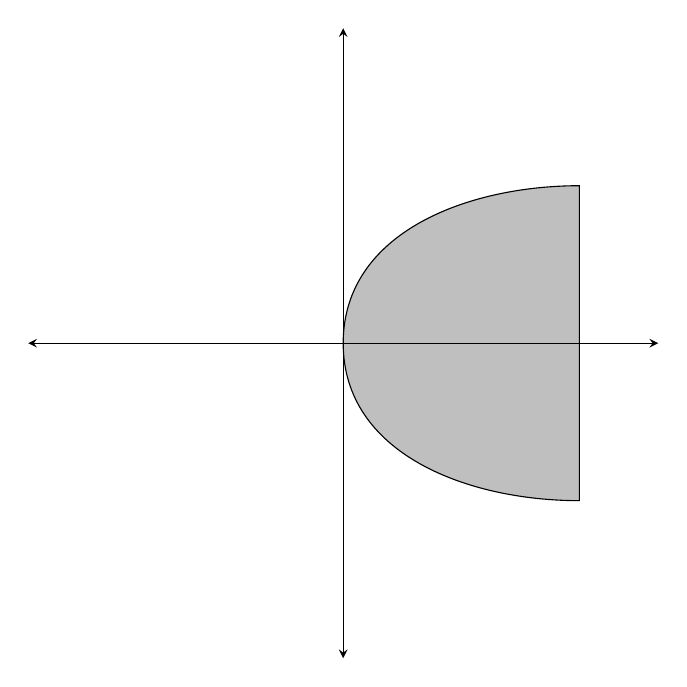
\begin{tikzpicture}
	\draw [fill = lightgray] (3,-2) [out = 180, in = -90] to (0,0) [out = 90, in = 180] to (3,2) -- cycle;
		
	\begin{scope}[stealth-stealth]
		\draw (-4,0) -- (4,0);
		\draw (0,-4) -- (0,4);
	\end{scope}
\end{tikzpicture}

\begin{equation*}
	V = \pi \int\limits_{a}^{b} \left( f(x) \right)^2 \dif x
\end{equation*}

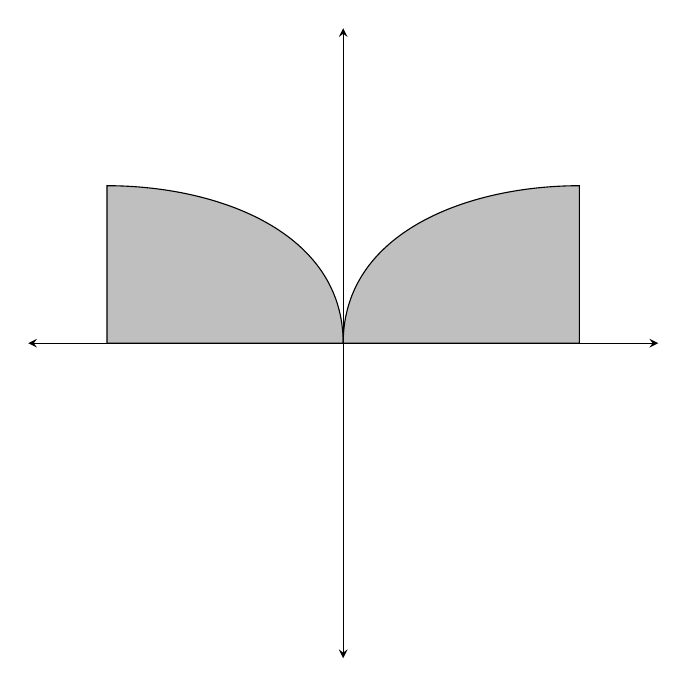
\begin{tikzpicture}
	\draw [fill = lightgray] (-3,2) [out = 0, in = 90] to (0,0) -- (-3,0) -- cycle;
	\draw [fill = lightgray](0,0) [out = 90, in = 180] to (3,2) -- (3,0) -- cycle;
		
	\begin{scope}[stealth-stealth]
		\draw (-4,0) -- (4,0);
		\draw (0,-4) -- (0,4);
	\end{scope}
\end{tikzpicture}

\begin{equation*}
	V = 2 \pi \int\limits_{a}^{b} x f(x) \dif x
\end{equation*}

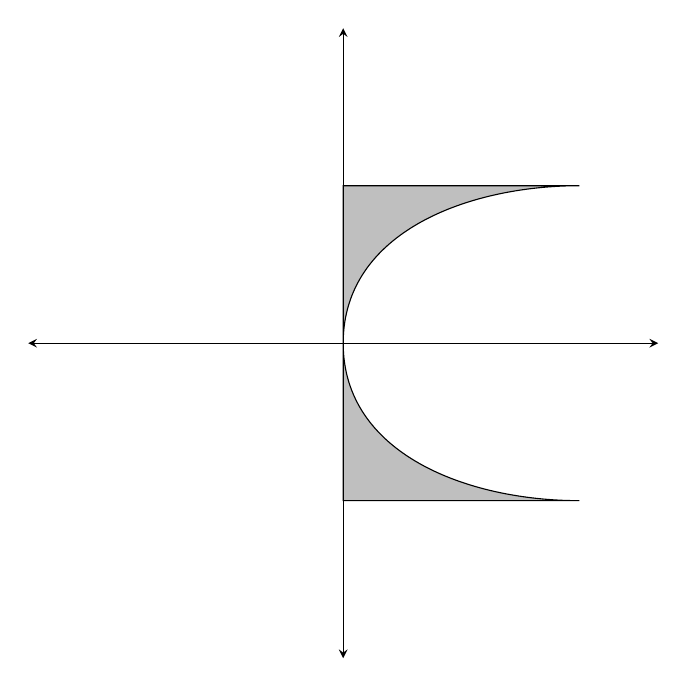
\begin{tikzpicture}
	\draw [fill = lightgray] (3,-2) [out = 180, in = -90] to (0,0) -- (0,-2) -- cycle;
	\draw [fill = lightgray] (0,0) [out = 90, in = 180] to (3,2) -- (0,2) -- cycle;
		
	\begin{scope}[stealth-stealth]
		\draw (-4,0) -- (4,0);
		\draw (0,-4) -- (0,4);
	\end{scope}
\end{tikzpicture}

\begin{equation*}
	V = 2 \pi \int\limits_{a}^{b} y f(y) \dif y
\end{equation*}

\subsection{Improper Integrals}

\subsubsection{Direct Comparison Tests}

\begin{theorem}[First comparison test]
	Let $f(x)$ and $g(x)$ be two functions defined on $[a, +\infty)$ and Riemann integrable over $[a, t], \forall t \geq a$. Assume that $\exists b \geq a$, s.t. $f(x) \geq g(x) \geq 0, \forall x \geq b$. Then,
	\begin{enumerate}
		\item if $\int\limits_{a}^{+\infty} f(x) \dif x$ converges, then $\int\limits_{a}^{+\infty} g(x) \dif x$ converges.
		\item if $\int\limits_{a}^{+\infty} g(x) \dif x$ diverges, then $\int\limits_{a}^{+\infty} f(x) \dif x$ diverges.
	\end{enumerate}
\end{theorem}

\begin{theorem}[Second comparison test]
	Assume $f(x) \geq g(x) \geq 0, \forall x \in (a,b)$. Assume that $f$, $g$ are not bounded in a neighbourhood of $b$ but integrable on intervals of the type $[a, t]$ for $a < t < b$. Assume that 
	\begin{equation*}
		\lim\limits_{x \to b^-} \dfrac{f(x)}{g(x)} = l > 0
	\end{equation*}
	Then, \[\int\limits_{a}^{b} f(x) \dif x\]and \[\int\limits_{a}^{b} g(x) \dif x\] converge or diverge simultaneously.
\end{theorem}

\section{Multi-variable Functions}

\begin{theorem}[Existence of limits]
	Let $\exists g(r,\theta)$, s.t. $f(x,y) = g(r, \theta)$. Then, if it exists, 
	\begin{equation*}
		\lim\limits_{(x,y) \to (0,0)} f(x,y) = \lim\limits_{r \to 0} g(r, \theta)
	\end{equation*}
\end{theorem}

\begin{definition}[Critical point]
	If both of $f_x(a,b)$ and $f_y(a,b)$ are zero, or if at least one of them does not exist, then $(a,b)$ is said to be a critical point.
\end{definition}

\begin{theorem}[A necessary condition for local extrema existence]
	If the function $z = f(x, y)$ has a local extrema at the point $(a, b)$ and $\exists f_x (a, b)$ and $\exists f_y (a, b)$ then $f_x (a, b) = f_y (a, b) = 0$
\end{theorem}

\begin{theorem}[A sufficient condition for local extrema point]
	Assume that there exist second order partial derivates of $z = f(x,y)$, they are continuous on some open neighbourhood of $(a,b)$ and $f_x(a,b) =f_y(a,b) = 0$. Denote 
	\begin{equation*}
	D(a, b) = f_{xx}(a,b) f_{yy}(a,b) - \left( f_{xy}(a,b) \right)^2
	\end{equation*}
	\begin{enumerate}
		\item If $D(a,b) > 0$ and $f_{xx} < 0$ then $(a,b)$ is a local maximum point.
		\item If $D(a,b) > 0$ and $f_{xx} > 0$ then $(a,b)$ is a local minimum point.
		\item If $D(a,b) < 0$ then $(a,b)$ is called a saddle point.
	\end{enumerate}
\end{theorem}

\begin{example}
	Find all critical points of 
	\begin{equation*}
	z = f(x,y) = x^4 + y^4 - 4xy + 1
	\end{equation*}
	and classify them.
\end{example}

\begin{solution}
	\begin{align*}
		f_x(x,y) &= 4x^3 - 4y\\
		f_y(x,y) &= 4y^3 - 4x
	\end{align*}
	For critical points,
	\begin{align*}
		f_x(x,y) &= 0\\
		f_y(x,y) &= 0
	\end{align*}
	Solving, $(0,0)$, $(1,1)$, $(-1,-1)$ are critical points.
	\begin{align*}
		f_{xx}(x,y) &= 12x^2\\
		f_{xy}(x,y) &= -4\\
		f_{yy}(x,y) &= 12y^2\\
		\therefore D(x,y) &= 144 x^2 y^2 - 16
	\end{align*}
	For $(0,0)$,
	\begin{align*}
		D &= -16
	\end{align*}
	Therefore, $(0,0)$ is a saddle point.\\
	For $(1,1)$,
	\begin{align*}
		D &= 144-16
	\end{align*}
	Therefore, $(1,1)$ is a local minimum point.\\
	For $(-1,-1)$,
	\begin{align*}
		D &= 144-16
	\end{align*}
	Therefore, $(-1,-1)$ is a local minimum point.\\
\end{solution}


\begin{definition}[Gradient]
	\begin{align*}
		\nabla f(x, y, z) &= (f_x(x, y, z), f_y(x, y, z), f_z(x, y, z)) \neq 0
	\end{align*}
\end{definition}

\begin{theorem}
	If $F(x, y, z)$ is differentiable at some point $P_0 (x_0, y_0, z_0)$ on the surface, then the tangent plane $\alpha$ to the surface at the point can be calculated by the formula
	\begin{align*}
	F_x (P_0) (x - x_0) + F_y (P_0) (y - y_0) + F_z (P_0) (z - z_0) &= 0
	\end{align*}
\end{theorem}

\subsection{Lagrange Multipliers}
To find the extrema of $f(x,y,z)$ subject to the constraint $g(x,y,z) = k$, solve
\begin{align*}
	\nabla f(x,y,z) &= \lambda \nabla g(x,y,z)\\
	g(x,y,z) &= k
\end{align*}

\section{Double Integrals}

\begin{theorem}[Area of a surface]
	If $f_x(x,y)$ and $f_y(x,y)$ are continuous in $D$, then the area of the surface $\sigma : z = f(x,y)$ above $D$ is equal to 
	\begin{equation*}
		S(\sigma) = \iint\limits_{D} \sqrt{1 + \left( f_x(x,y) \right)^2 + \left( f_y(x,y) \right)^2} \dif A
	\end{equation*}
\end{theorem}

\begin{definition}[Centre of mass]
	If $\rho(x,y)$ is the density function of a thin body,
	\begin{align*}
		m &= \iint\limits_{D} \rho(x,y) \dif A
	\end{align*}
	\begin{align*}
		(x_{\text{COM}}, y_{\text{COM}}) &= \left( \dfrac{M_y}{m}, \dfrac{M_x}{m} \right)\\
		\intertext{where}
		M_x &= \iint\limits_{D} y \rho(x,y) \dif A\\
		M_y &= \iint\limits_{D} x \rho(x,y) \dif A\\
	\end{align*}
\end{definition}

\begin{definition}[Domain of the first kind]
	A domain $D$ is said to be the domain of the first kind if there exist continuous functions $f_1(x)$ and $f_2(x)$, s.t.
	\begin{align*}
	D_{\textnormal{I}} &= \{(x,y) | a \leq x \leq b, f_1(x) \leq y \leq f_2(x)\}
	\end{align*}
\end{definition}

\begin{theorem}
	If $f(x,y)$ is continuous in $D_{\textnormal{I}}$, then
	\begin{align*}
		\iint\limits_{R} f(x,y) \dif A &= \int\limits_{a}^{b} \int\limits_{f_1(x)}^{f_2(x)} f(x,y) \dif y \dif x
	\end{align*}
\end{theorem}

\begin{definition}[Domain of the second kind]
	A domain $D$ is said to be the domain of the second kind if there exist continuous functions $g_1(y)$ and $g_2(y)$, s.t.
	\begin{align*}
		D_{\textnormal{II}} &= \{(x,y) | c \leq y \leq d, g_1(y) \leq x \leq g_2(y)\}
	\end{align*}
\end{definition}

\begin{theorem}
	If $f(x,y)$ is continuous in $D_{\textnormal{II}}$, then
	\begin{align*}
		\iint\limits_{R} f(x,y) \dif A &= \int\limits_{c}^{d} \int\limits_{g_1(y)}^{g_2(y)} f(x,y) \dif x \dif y
	\end{align*}
\end{theorem}

\section{Triple Integrals}

\begin{example}
	Find $\displaystyle \iiint\limits_{E} x^2 + y^2 + z^2 \dif V$ where $E$ is bounded by $x = 0$, $y = 0$, $z = 0$ and $x + y + z = a, a > 0$.
\end{example}

\begin{solution}
	~\\
	\begin{tikzpicture}
	\def\a{2};
	
	\begin{scope}[-stealth]
		\draw (0,0,0) -- ({\a+1},0,0);
		\draw (0,0,0) -- (0,{\a+1},0);
		\draw (0,0,0) -- (0,0,{\a+1});
	\end{scope}
	
	\begin{scope}
		\draw (\a,0,0) -- (0,\a,0) -- (0,0,\a) -- cycle;
	\end{scope}
	\end{tikzpicture}\\
	Therefore,
	\begin{align*}
		\iiint\limits_{E} x^2 + y^2 + z^2 \dif V &= \int\limits_{0}^{a} \int\limits_{0}^{a - x} \int\limits_{0}^{a - x - y} x^2 + y^2 + z^2 \dif z \dif y \dif x
	\end{align*}
\end{solution}

\begin{example}
	Calculate $\displaystyle \iiint\limits_{E} x e^z \dif V$ where $E$ is bounded by $z = x^2 + y^2$ and $z = 8 - x^2 - y^2$.
\end{example}

\begin{solution}
	The two boundaries intersect at $x^2 + y^2 = 4$. Therefore the projection of the volume is the circle.\\
	Therefore,
	\begin{align*}
		\iiint\limits_{E} x e^z \dif V &= \int\limits_{-2}^{2} \int\limits_{-\sqrt{4 - x^2}}^{\sqrt{4 - x^2}} \int\limits_{x^2 + y^2}^{8 - x^2 - y^2} x e^z \dif z \dif y \dif x
	\end{align*}
\end{solution}

\section{Line Integrals of Scalar Functions}

\begin{definition}[Smooth curve]
	Let $C$ be given parametrically as
	\begin{equation*}
		\overline{r} (t) = \left( x(t), y(t) \right) \quad t : a \to b
	\end{equation*}
	The curve is said to be smooth if 
	\begin{equation*}
		\overline{r}'(t) = \left( x'(t), y'(t) \right)
	\end{equation*}
	is a continuous function on $[a,b]$, $\overline{r}'(t) \neq \overline{0}$ on $(a,b)$ and $\overline{r}'(t)$ is also continuous on $(a,b)$.
\end{definition}

\begin{theorem}
	If $f(x,y)$ is continuous and $C$ is smooth, then
	\begin{equation*}
		\int\limits_{C} f(x,y) \dif s = \int\limits_{a}^{b} f(x(t), y(t)) \sqrt{\left( x'(t) \right)^2 + \left( y'(t) \right)^2} \dif t
	\end{equation*}
\end{theorem}

\begin{example}
	Calculate $\displaystyle \int\limits_{C} x^2 + y^2 \dif s$ where $C$ is a circle of radius 2.
\end{example}

\begin{solution}
	\begin{align*}
		\int\limits_{C} x^2 + y^2 \dif s &= \int\limits_{0}^{2 \pi} \left( (2 \cos t)^2 + (2 \sin t)^2 \right) \cdot 2 \dif t\\
		&= 16 \pi
	\end{align*}
\end{solution}

\section{Line Integrals of Vector Functions}

\begin{definition}[Line integral of vector function]
	\begin{align*}
		W &= \int\limits_{C} \overline{F} \cdot \hat{T} \dif s\\
		&= \int\limits_{C} \overline{F} \cdot \dif \overline{z}\\
		&= \int\limits_{C} P \dif x + Q \dif y + R \dif z
	\end{align*}
\end{definition}	

\begin{example}
	Find the work $W$ done by the force $\overline{F}(x,y) = (x, xy)$ over the curve $C : \overline{r}(t) = (2 \cos t, 2 \sin t) , t : \pi \to 2 \pi$.
\end{example}

\begin{solution}
	\begin{align*}
		W &= \int\limits_{C} \overline{F} \cdot \hat{T} \dif s\\
		&= \int\limits_{\pi}^{2 \pi} \left( 2 \cos t (-2 \sin t) + 2 \cos t \cdot 2 \sin t \cdot 2 \cos t \right) \dif t\\
		&= \int\limits_{\pi}^{2 \pi} \left( - 2 \sin (2t) + 8 \cos^2 t \sin t \right) \dif t\\
		&= \left. \cos (2t) - \dfrac{8}{3} \cos^3 t \right\rvert_{\pi}^{2 \pi}\\
		&= \left( 1 - \dfrac{8}{3} \right) - \left( 1 + \dfrac{8}{3} \right)\\
		&= -\dfrac{16}{3}
	\end{align*}
\end{solution}

\begin{example}
	Calculate $\displaystyle \int\limits_{C} \dfrac{x}{y} \dif x + \dfrac{y - x}{x} \dif y$ where $C$ is the path over the parabola $y = x^2$ from $(2,4)$ to $(1,1)$.
\end{example}

\begin{solution}
	\begin{align*}
		\int\limits_{C} \left( \dfrac{x}{y}, \dfrac{y - x}{x} \right) \dif r &= \int\limits_{2}^{1} \left( \dfrac{t}{t^2} + \dfrac{t^2 - t}{t} \right) \cdot (1, 2t) \dif t\\
		&= \int\limits_{2}^{1} \left( \dfrac{1}{t} + (t - 1) \cdot 2t \right) \dif t\\
		&= \left. \ln t + \dfrac{2 t^3}{3} - t^2 \right|_{2}^{1}\\
		&= \ln \dfrac{1}{2} + \dfrac{2}{3} - \dfrac{16}{3} - 1 + 4\\
		&= 3 - \dfrac{14}{3} - \ln 2\\
		&= \dfrac{5}{3} - \ln 2
	\end{align*}
\end{solution}

\begin{theorem}[The Fundamental Theorem of Line Integrals]\label{The Fundamental Theorem of Line Integrals}
	Let $C$ be a smooth curve in $\mathbb{R}^2$ or $\mathbb{R}^3$ given parametrically by $\overline{r}(t)$, $t : a \to b$. Let $f$ be a continuous function of $(x,y)$ or $(x,y,z)$ respectively, on $C$ and $\nabla f$ be a continuous vector function in a connected domain $D$ which contains $C$. Then
	\begin{align*}
		W &= \int\limits_{C} \nabla f \cdot \hat{T} \dif s\\
		&= f(r(b)) - f(r(a))\\
		&= f(B) - f(A)
	\end{align*}
\end{theorem}

\begin{definition}[Simple curve]
A curve $C$ is called a simple curve if it does not intersect itself.
\end{definition}

\begin{definition}[Domain]
	A domain $D \subset \mathbb{R}^2$ is called connected if for any two points from $D$, the is a path $C$ which connects the points and remains in $D$.
\end{definition}

\begin{definition}[Simple connected domain]
	A connected domain $D \subset \mathbb{R}^2$ is called simple connected if any simple closed curve from $D$ contains inside itself only points in $D$.
\end{definition}

\begin{theorem}
	If
	\begin{equation*}
		\overline{F}(x,y) = \left( P(x,y), Q(x,y) \right) = \nabla f(x,y)
	\end{equation*}
	is the conservative vector field in a connected domain $D$, where there exist first order partial derivatives of $P$ and $Q$ continuous in $D$, then
	\begin{align*}
		P_y(x,y) &= Q_x(x,y) &\forall (x,y) \in D
	\end{align*}
\end{theorem}

\begin{theorem}
	Let
	\begin{equation*}
	\overline{F}(x,y) = \left( P(x,y), Q(x,y) \right)
	\end{equation*}
	be a vector field in an open, simple connected domain $D$. If there exist first order partial derivatives of $P$ and $Q$ which are continuous in $D$, and
	\begin{align*}
		P_y(x,y) &= Q_x(x,y) &\forall (x,y) \in D
	\end{align*}
	Then, $\exists f(x,y)$ s.t.
	\begin{equation*}
		\overline{F}(x,y) = \nabla f(x,y)
	\end{equation*}
	i.e. $\overline{F}$ is a conservative vector field.
\end{theorem}

\begin{example}
	If 
	\begin{equation*}
		\overline{F}(x,y) = (3 + 2 x y, x^2 - 3 y^2)
	\end{equation*}
	a conservative vector field? If yes, find $f(x,y)$, s.t.
	\begin{equation*}
		\overline{F}(x,y) = \nabla f(x,y)
	\end{equation*}
	and find the work done by the force $\overline{F}(x,y)$ over the curve
	\begin{align*}
		\overline{r}(t) &= (e^t \sin t, e^t \cos t) & t : 0 \to \pi
	\end{align*}
\end{example}

\begin{solution}
	\begin{align*}
		P(x,y) &= 3 + 2xy\\
		\therefore P_y &= 2x\\
		Q(x,y) &= x^2 - 3 y^2\\
		\therefore Q_x &= 2x\\
		\therefore P_y &= Q_x
	\end{align*}
	Therefore, $\overline{F}(x,y)$ is a conservative vector field.
	\begin{align*}
		f_x &= P\\
		&= 3 + 2 x y\\
		\therefore f &= 3x + x^2 y + c(y)\\
		\therefore f_y &= x^2 + c'(y)\\
		\intertext{Comapring with $f_y = Q$,}
		c'(y) &= -3 y^3\\
		\therefore c(y) &= - y^3 + c\\
		\therefore f(x,y) &= 3x + x^2 y - y^3 + c
	\end{align*}
	By the definition of work,
	\begin{align*}
		W &= \int\limits_{C} \overline{F} \cdot \hat{T} \dif s\\
		&= \int\limits_{a}^{b} \left( P(\overline{r}(t)) x'(t) + Q(\overline{r}(t)) y'(t) \right) \dif t
	\end{align*}
	Alternatively, using \nameref{The Fundamental Theorem of Line Integrals},
	\begin{align*}
		W &= \int\limits_{C} \overline{F} \cdot \hat{T} \dif s\\
		&= \int\limits_{C} \nabla d \cdot \hat{T} \dif s\\
		&= f(\overline{r}(\pi)) - f(\overline{r}(0))\\
		&= f(0, -e^{\pi}) - f(0, 1)\\
		&= -(-e^{\pi})^3 - (-1)^3\\
		&= e^{3 \pi} + 1
	\end{align*}
\end{solution}

\begin{theorem}[Green's Theorem]\label{Green's Theorem}
	Let $C$ be a piecewise smooth, simple, and closed curve in $\mathbb{R}^2$ with positive orientation. Let $D$ be a domain bounded by $C$. If there exist continuous first order partial derivatives of $P(x,y)$ and $Q(x,y)$ in an open domain which contains $D$, then
	\begin{equation*}
		W = \int\limits_{C} \overline{F} \cdot \hat{T} \dif s = \int\limits_{C} P \dif x + Q \dif y = \iint\limits_{D} (Q_x - P_y) \dif A
	\end{equation*}
\end{theorem}

\begin{remark}
	\nameref{Green's Theorem} is also true for domains with holes.
\end{remark}

\begin{example}
	Find the work done by the force 
	\begin{equation*}
		\overline{F}(x,y) = (x^4, xy)
	\end{equation*}
	over the path 
	\begin{equation*}
		C = C_1 \cup C_2 \cup C_3
	\end{equation*}
	\begin{tikzpicture}[scale = 2]
		\begin{scope}[stealth-stealth, lightgray]
			\draw (-1,0) -- (2,0);
			\draw (0,-1) -- (0,2);
		\end{scope}
		
		\begin{scope}[-stealth, thick]
			\draw (0,0) -- (1,0) node [midway, below] {$C_1$};
			\draw (1,0) -- (0,1) node [midway, above right] {$C_2$};
			\draw (0,1) -- (0,0) node [midway, left] {$C_3$};
		\end{scope}
		
		\node [below left] at (0,0) {$0$};
		\node [below] at (1,0) {$1$};
		\node [left] at (0,1) {$1$};
	\end{tikzpicture}
\end{example}

\begin{solution}
	By \nameref{Green's Theorem},
	\begin{align*}
		W &= \int\limits_{C} P \dif x + Q \dif y \\
		&= \iint\limits_{D} (Q_x - P_y) \dif A\\
		&= \iint\limits_{D} (y - 0) \dif A\\
		&= \int\limits_{0}^{1} \int\limits_{0}^{1 - x} y \dif y \dif x\\
		&= \dfrac{1}{6}
	\end{align*}
\end{solution}

\begin{example}
	Calculate $\displaystyle \int\limits_{C} \overline{F} \cdot \hat{T} \dif s$ when
	\begin{equation*}
		\overline{F} = \left( -\dfrac{y}{x^2 + y^2} , \dfrac{x}{x^2 + y^2} \right)
	\end{equation*}
	and $C$ is a simple, closed, piecewise smooth curve with positive orientation which does not pass through $(0,0)$.
\end{example}

\begin{solution}
	\begin{align*}
		P &= \dfrac{y}{x^2 + y^2}\\
		Q &= \dfrac{x}{x^2 + y^2}
	\end{align*}
	Therefore,
	\begin{align*}
		P_y &= -\dfrac{(x^2 + y^2) - y \cdot 2y}{(x^2 + y^2)^2}\\
		&= \dfrac{y^2 - x^2}{(x^2 + y^2)^2}\\
		Q_x &= \dfrac{(x^2 + y^2) - x \cdot 2x}{(x^2 + y^2)^2}
	\end{align*}
	If $(0,0) \notin D$, \nameref{Green's Theorem} is applicable.\\
	Therefore,
	\begin{align*}
		\int\limits_{C} \overline{F} \cdot \hat{T} \dif s &= \iint\limits_{D} (Q_x - P_y) \dif A\\
		&= 0
	\end{align*}
	If $(0,0) \in D$, \nameref{Green's Theorem} is not applicable as $P_y$ and $Q_x$ are not continuous in $D$.\\
	Let $C_1$ be a circle of radius $a$, with the same orientation as $C$. Let $\widetilde{C} = C \cup (-C_1)$. \nameref{Green's Theorem} can be applied on the domain $D \setminus D_1$ which is enclosed by $\widetilde{C}$.
	\begin{align*}
		\int\limits_{C \cup (-C_1)} P \dif x + Q \dif y &= \iint\limits_{D \setminus D_1} (Q_x - P_y) \dif A\\
		&= 0\\
		\int\limits_{C} P \dif x + Q \dif y + \int\limits_{-C_1} P \dif x + Q \dif y &= 0
	\end{align*}
	Therefore,
	\begin{align*}
		\int\limits_{C} P \dif x + Q \dif y &= \int\limits_{C_1} P \dif x + Q \dif y\\
		&= \quad \int\limits_{0}^{2 \pi} P\left( x(t), y(t) \right) x'(t) \dif t\\
		&\quad+ \int\limits_{0}^{2} Q\left( x(t), y(t) \right) \dif t\\
		&= \int\limits_{0}^{2 \pi} (\sin^2 t + \cos^2 t) \dif t\\
		&= 2 \pi
	\end{align*}
\end{solution}

\begin{example}
	Calculate $\displaystyle \int\limits_{C} -2e^{2x - y} \cos y \dif x + \left( e^{2x - y} (\sin y + \cos y) + 2xy \right) \dif y$ when $C$ is the half ellipse $\left\lbrace \dfrac{x^2}{4} + y^2 = 1, y \geq 0 \right\rbrace$ oriented from the point $(2,0)$ to the point $(-2,0)$.
\end{example}

\begin{solution}
	~\\
	\begin{tikzpicture}
	\begin{scope}[stealth-stealth, lightgray]
		\draw (-3,0) -- (3,0);
		\draw (0,-1) -- (0,2);
	\end{scope}
	
	\draw [thick, -stealth] (2,0) arc (0:90:2 and 1) node[above, near end] {$C$};
	\draw [thick] (0,1) arc (90:180:2 and 1);
	
	\draw [-stealth] (-2,0) -- (0,0) node [near end, below] {$C_1$};
	\draw (0,0) -- (2,0);
	\end{tikzpicture}\\
	Let $C_1$ be the line segment as shown.
	\begin{align*}
		P &= -2e^{2x - y} \cos y\\
		Q &= e^{2x - y} (\sin y + \cos y) + 2xy
	\end{align*}
	Therefore,
	\begin{align*}
		P_y &= 2e^{2x - y} \cos y + 2e^{2x - y} \sin y \\
		&= 2 e^{2x - y} (\cos y + \sin y)\\
		Q_x &= 2e^{2x - y} (\sin x + \cos y) + 2y
	\end{align*}
	The domain is of the first kind.
	\begin{align*}
		\int\limits_{C} P \dif x + Q \dif y &= \int\limits_{C} P \dif x + Q \dif y + \int\limits_{C_1} P \dif x + Q \dif y\\
		&\quad - \int\limits_{C_1} P \dif x + Q \dif y\\
		&= \int\limits_{C \cup C_1} P \dif x + Q \dif y - \int\limits_{C_1} P \dif x + Q \dif y\\
		&= \iint\limits_{D} (Q_x - P_y) \dif A - \int\limits_{C_1} P \dif x + Q \dif y
	\end{align*}
\end{solution}

\end{multicols}

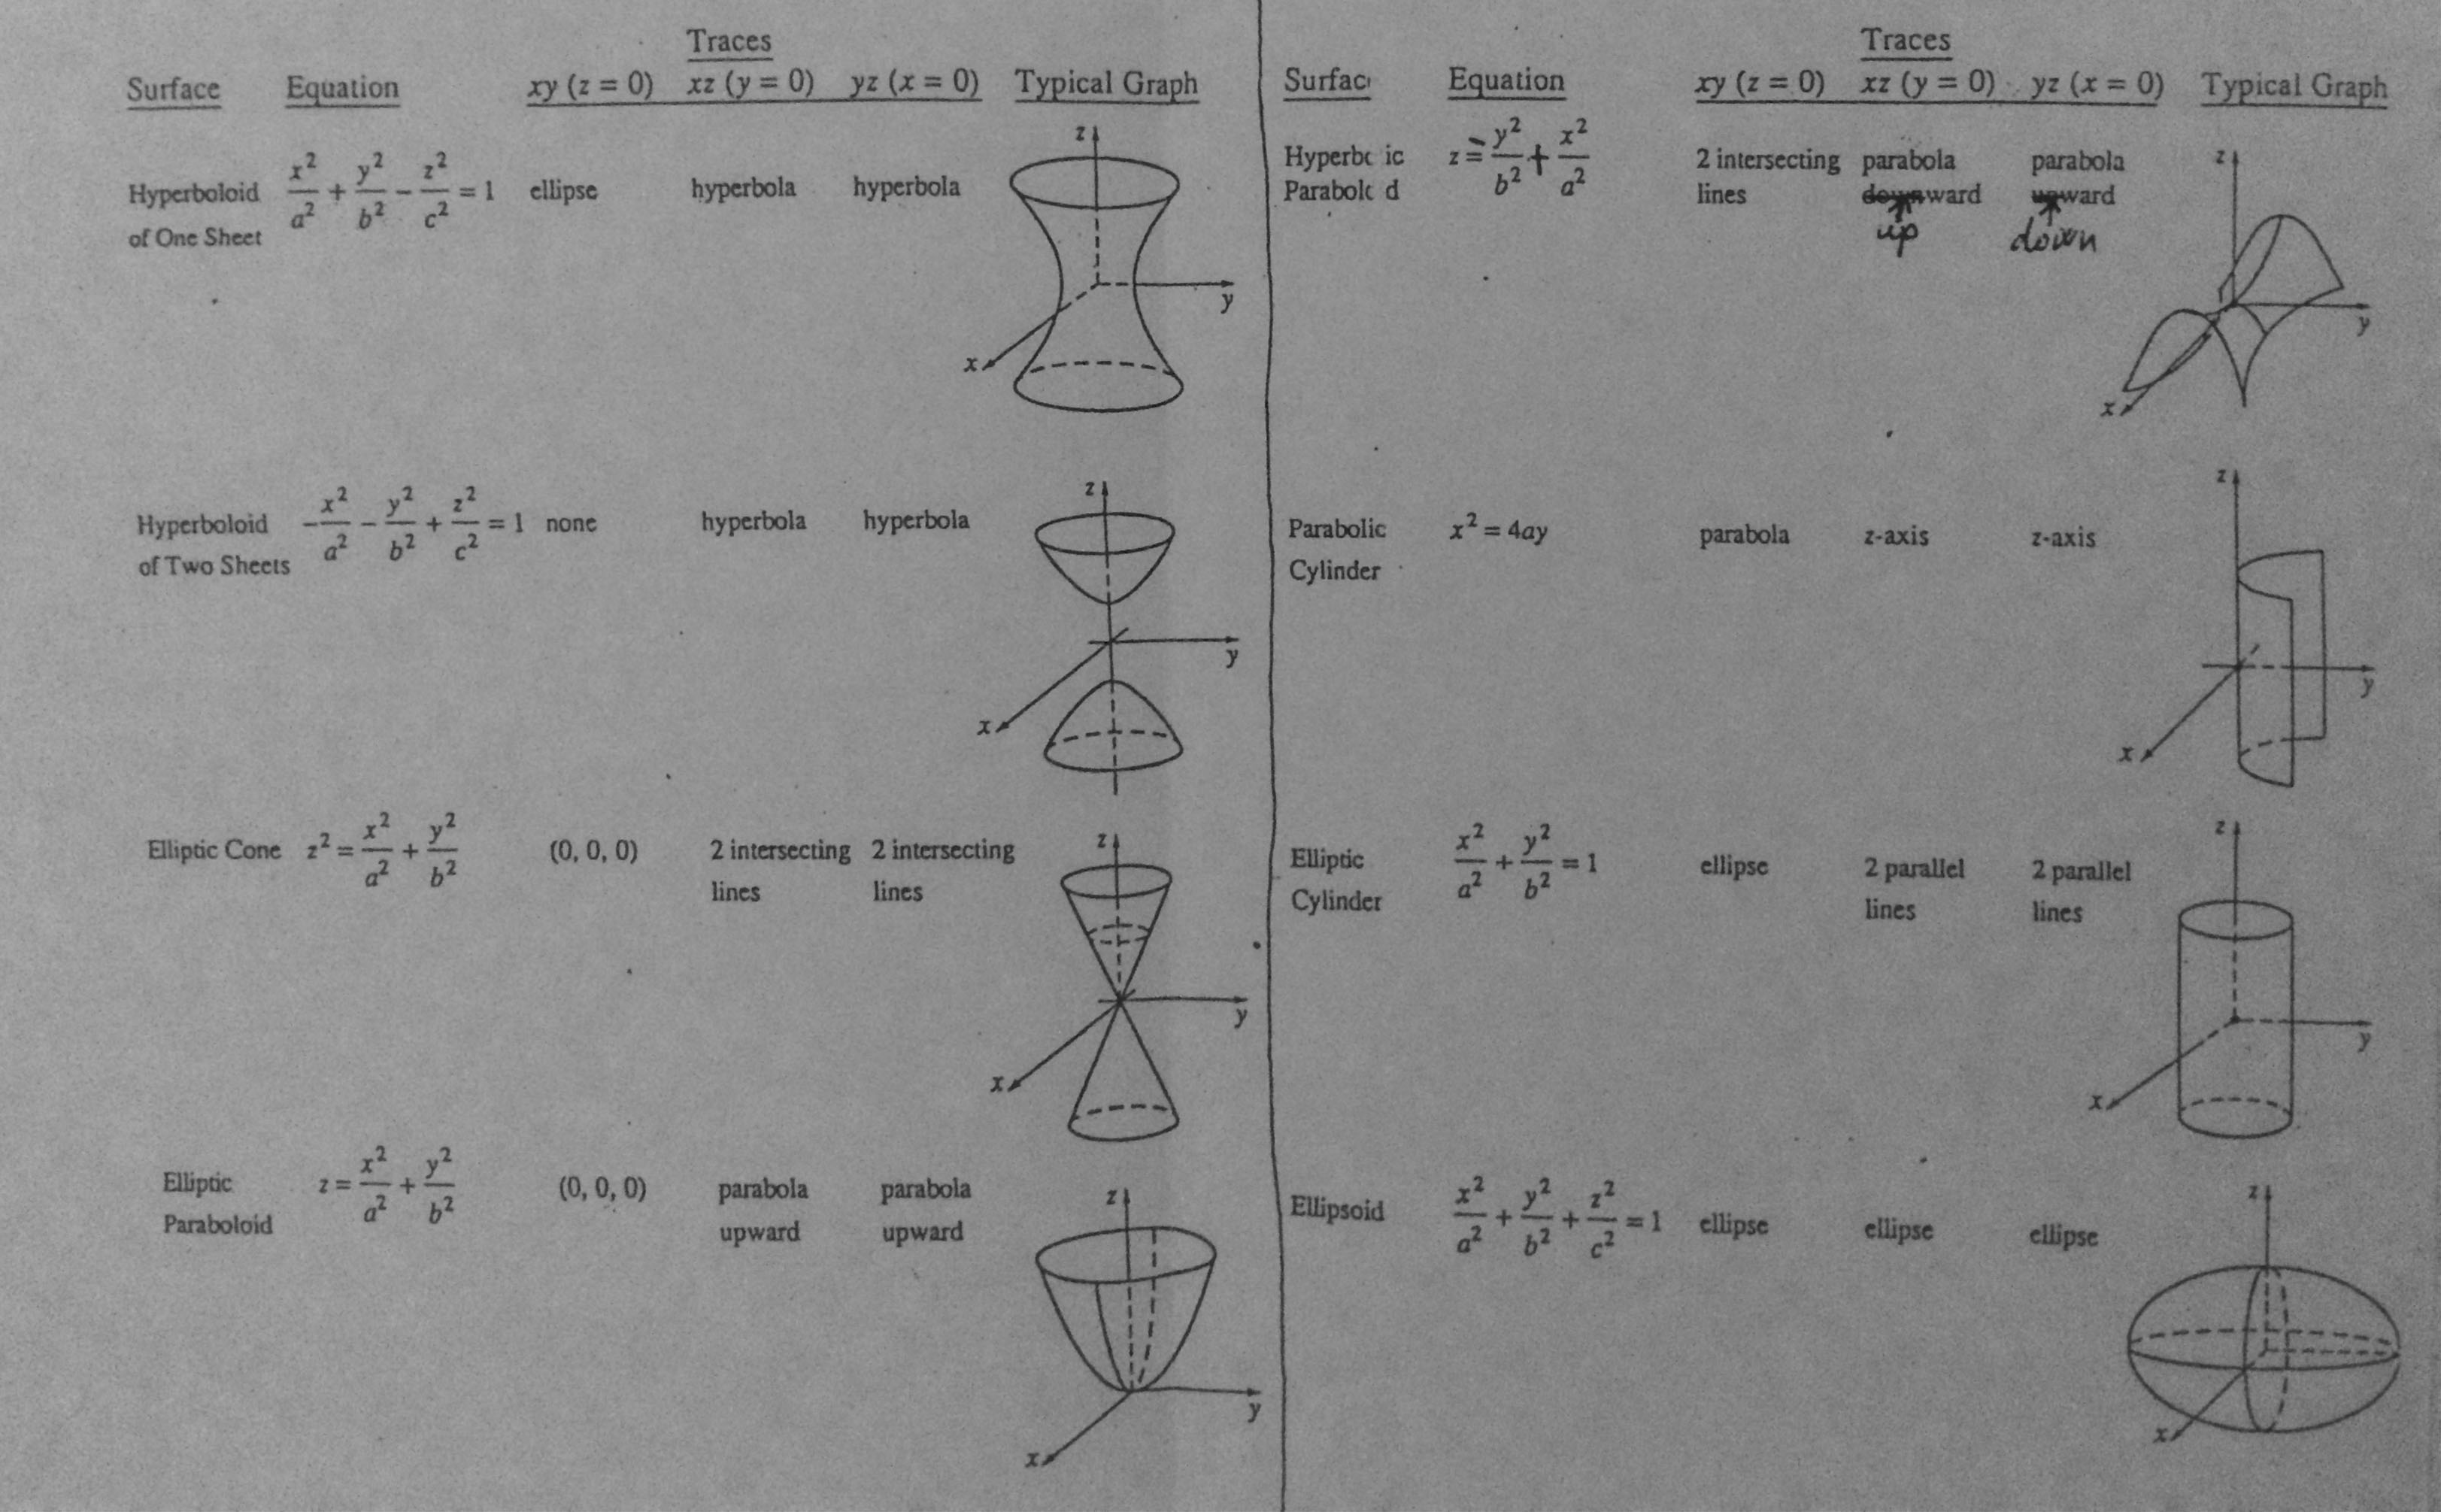
\includegraphics[width = \textwidth]{IMG_5498_bw.JPG}

\end{document}